% Ver readme, hay dependencias necesarias para instalar. 

\documentclass{article}
\usepackage{graphicx}

\begin{document}

\section{Model}


\section{Gráfico}

Based on USDT adoption data as a proxy for stablecoin adoption between 2019 and 2024, countries can be classified into three distinct groups according to their level of adoption. In the high adoption group, countries such as Turkey, Nigeria, Argentina, and Ukraine stand out, with USDT adoption rates above 80\% during this period. In the moderate adoption group are countries such as Brazil, Russia, and Australia, with adoption rates ranging between 60\% and 80\%. Finally, the low adoption group includes countries such as Canada, the United States, Japan, and the United Kingdom, with USDT adoption rates below 60\%, indicating a lower level of integration of stablecoins into their financial systems.

In terms of the average year-on-year evolution between 2023 and 2024, a mixed trend in USDT adoption can be observed. Countries in the high adoption group, such as Nigeria and Ukraine, showed sustained growth with average annual rates above 10\%. On the other hand, countries with moderate adoption, such as Brazil and Australia, experienced moderate growth. In contrast, countries in the low adoption group, such as the United States and Japan, recorded negative or very low growth rates. 

The adoption of USDT as a proxy for stablecoin adoption shows differences between emerging market economies -EMEs- and advanced economies -AEs-. Within emerging market economies, two distinct groups can be identified: one with high adoption, which includes countries such as Turkey, Nigeria, and Argentina, and one with moderate adoption, represented by Brazil and Russia. Conversely, in advanced economies, adoption is predominantly moderate, with exceptions such as Australia, which shows more significant adoption but still not as extensive as in some emerging countries. 

\begin{figure}[h]
    \centering
    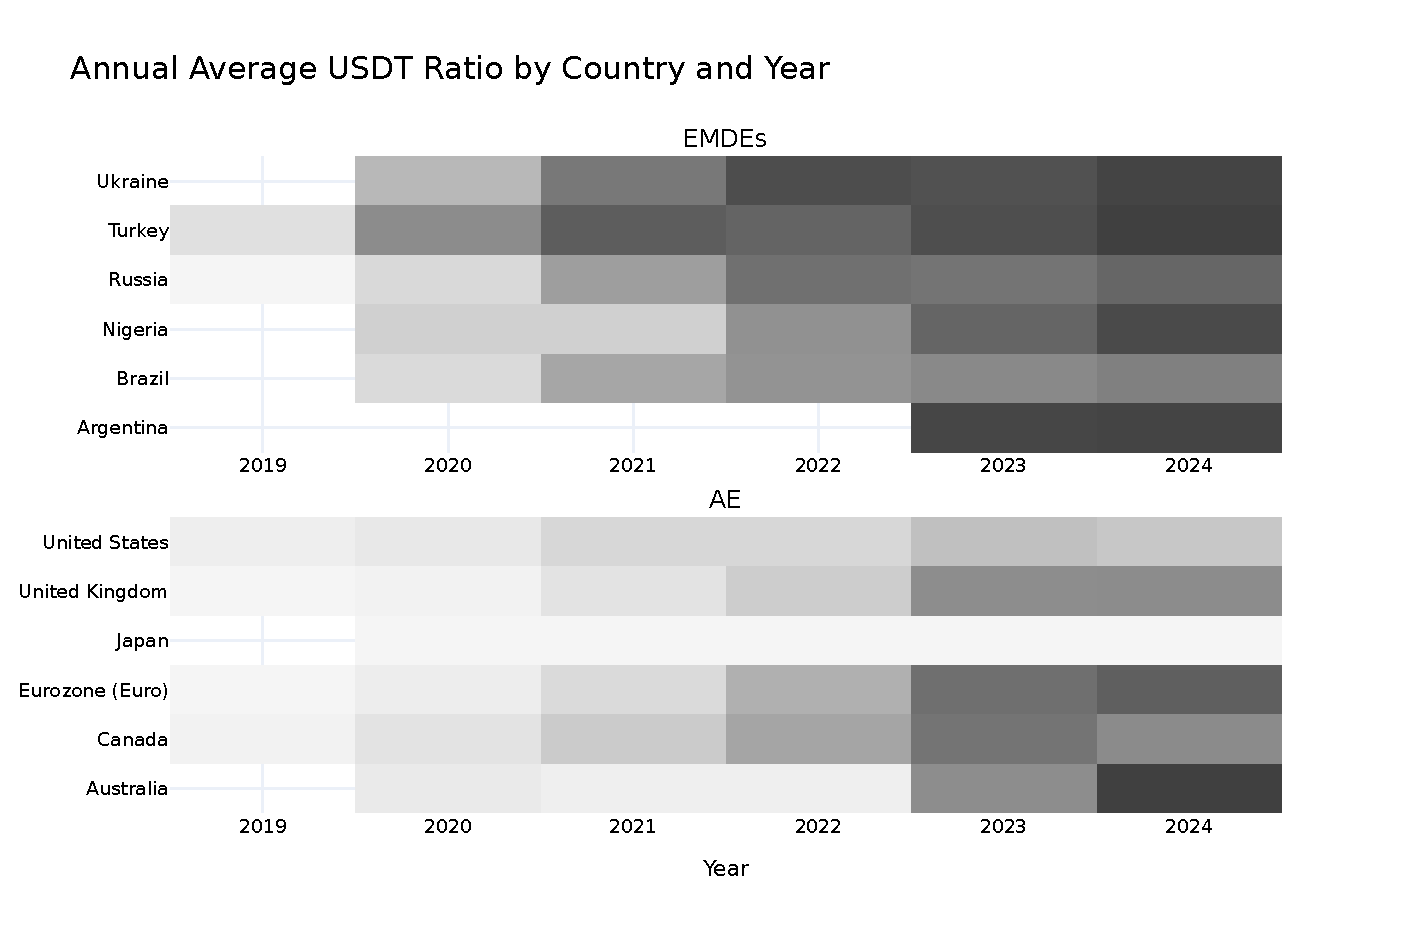
\includegraphics[width=1\textwidth]{graphs/usdt_ratio.pdf} % Asegúrate de tener un archivo grafico.pdf en la carpeta "graphs"
    \caption{Gráfico generado con Plotly}
    \label{fig:grafico}
\end{figure}

\end{document}